\chapter{Introduction}
\label{chapter:introduction}

\begin{chapquote}[2em]{Jan M. Pawlowski}
``There is no free lunch.''
\end{chapquote}

The experimental control of ultracold Fermi gases provides a powerful tool for studying strongly correlated quantum systems including the BCS-BEC crossover~\cite{Randeria2014} and Fermi polarons~\cite{Parish2023}. Understanding these exotic quantum phenomena is essential for the future development of high-temperature superconductors and quantum computers.

Various non-perturbative approaches, such as Quantum Monte Carlo (QMC) simulations \cite{Magierski2009,Prokofev2008}, selfconsistent T-matrix theory~\cite{Hanai2013,Pini2019} or the Luttinger-Ward formalism~\cite{Haussmann1999,Haussmann2007}, as well as Dyson-Schwinger equations (DSEs)~\cite{Boettcher2013,Diener2008} and functional Renormalization Group (fRG) methods~\cite{Diehl2006-2,Diehl2010} have been employed to describe strongly interacting fermions.

A central object of interest in real-time applications is the spectral function~\cite{Kallen1952,Lehmann1954} which encodes information about scattering properties and the energy spectrum of the system. Its determination requires knowledge of correlation functions at real frequencies. However, the approaches mentioned above are usually formulated in imaginary frequencies by construction or due to significantly reduced computational costs for the calculation of thermodynamic observables~\cite{Frank2018}. This leaves an ill-conditioned numerical problem when analytically continuing to real frequencies~\cite{Wink2020}.

Numerical reconstruction methods, such as Padé approximations~\cite{Schmidt2011} or the Maximum Entropy Method~\cite{Haussmann2009} have been utilized to obtain spectral functions from imaginary-time data. However, these techniques are plagued by large systematic uncertainties and cannot guarantee a correct result. Therefore, a direct real-time computation is favorable.

In this Thesis, functional methods are used to calculate spectral functions of ultracold Fermi gases directly in real frequencies without the need of numerical reconstruction methods. As a proof of principle, the selfconsistent real-time framework is applied to the well-known spin-balanced BCS-BEC crossover and the Fermi polaron problem. Previous results are verified and novel spectral functions are presented.

This work is organized as follows. In Chapter~\ref{chapter:functional-methods}, the functional description of Quantum Field Theories (QFTs) at finite temperature and the spectral representation of propagators are introduced briefly. In Chapter~\ref{chapter:ultracold-gases}, the theoretical background of ultracold Fermi gases is presented. In this context, the microscopic model of the theory and first mean-field considerations are discussed. The main part of this work is summarized in Chapter~\ref{chapter:bcs-bec-crossover} and deals with the spectral properties of the BCS-BEC crossover phase diagram, see Fig.~\ref{fig:crossover-phase-diagram}. In particular, the normal phase above the critical temperature is investigated in detail and a brief outlook towards the superfluid phase is given. Analytical and numerical results are discussed and compared to other works. In Chapter~\ref{chapter:fermi-polaron}, the selfconsistent functional approach is applied to the Fermi polaron problem and compared with previous works. Finally, in Chapter~\ref{chapter:conclusion}, important results are summarized and a small outlook for future work is given.


\begin{figure}[h]
\centering
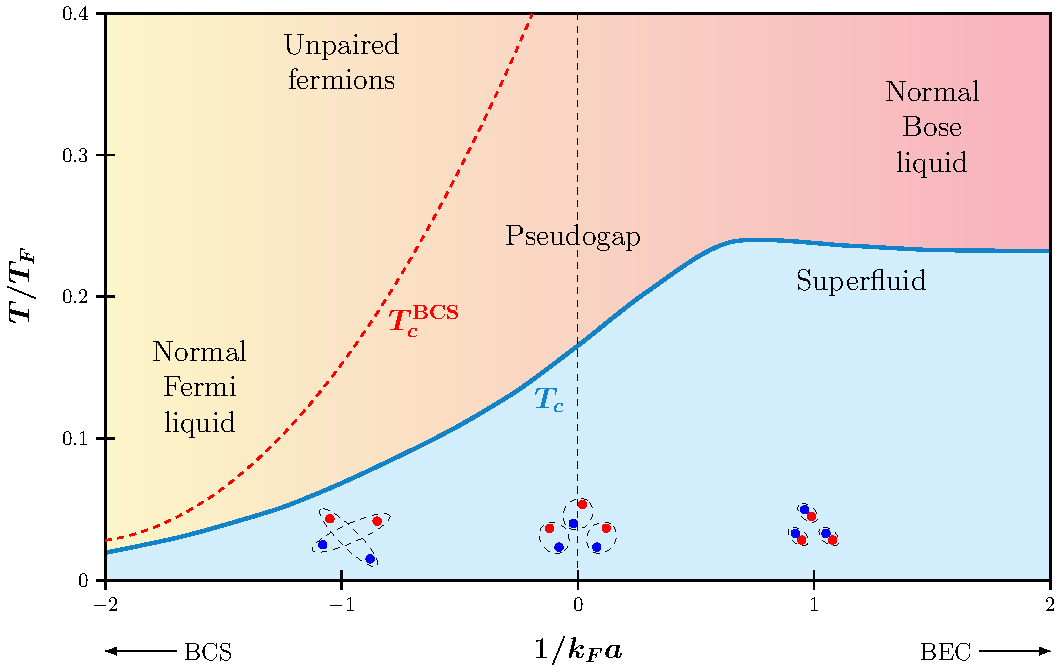
\includegraphics[width=0.75\linewidth]{figs/bcs-bec.pdf}
\caption[Phase diagram of the BCS-BEC crossover]{Phase diagram of the BCS-BEC crossover as a function of temperature $T/T_F$ and coupling strength $1/k_Fa$, where $T_F$ and $k_F$ is the Fermi temperature and momentum, respectively, and $a$ is the two-body scattering length. Inspired by~\cite{Randeria2014} with new results from~\cite{Haussmann2007}.}
\label{fig:crossover-phase-diagram}
\end{figure}


\section*{Notation and Units}

In this Thesis, natural units with $\hbar = c = k_B = 2m = 1$, where $m$ is the fermion mass, are used. All dimensionful quantities are measured in terms of the density $n$, or Fermi momentum $k_F=(3\pi^2n)^{1/3}$. Temperature and energy-like quantities are measured in terms of Fermi energy $T_F=\varepsilon_F=k_F^2$. Sometimes, dimensionful constants are reintroduced to remind the reader of the correct units. Three-vectors are denoted by bold letters. For the sake of simplicity, we use the same notation for the fields $\psi_{\sigma}$, with fermion species $\sigma=(\uparrow,\downarrow)$, and $\phi$ in the classical and effective action.

We use the integral conventions
\begin{align}
	\int_x = \int d^dx \quad \mathrm{and} \quad  \int_p = \int \frac{d^dp}{(2\pi)^d} \,.
\end{align}
